\section{Problemanalyse}
Problemanalysen tager udgangspunkt i nøgleproblemet spildtid jf. projektbeskrivelsen i appendikssektionen (\ref{appendix:projektbeskrivelse}). 


\subsection{Problemtræ}
Forneden har vi fremstillet et problemtræ, der viser nogle af årsagerne til tidsspild og nogle af virkningerne.
\begin{figure}[H]
    \centering
    \resizebox{\columnwidth}{!}{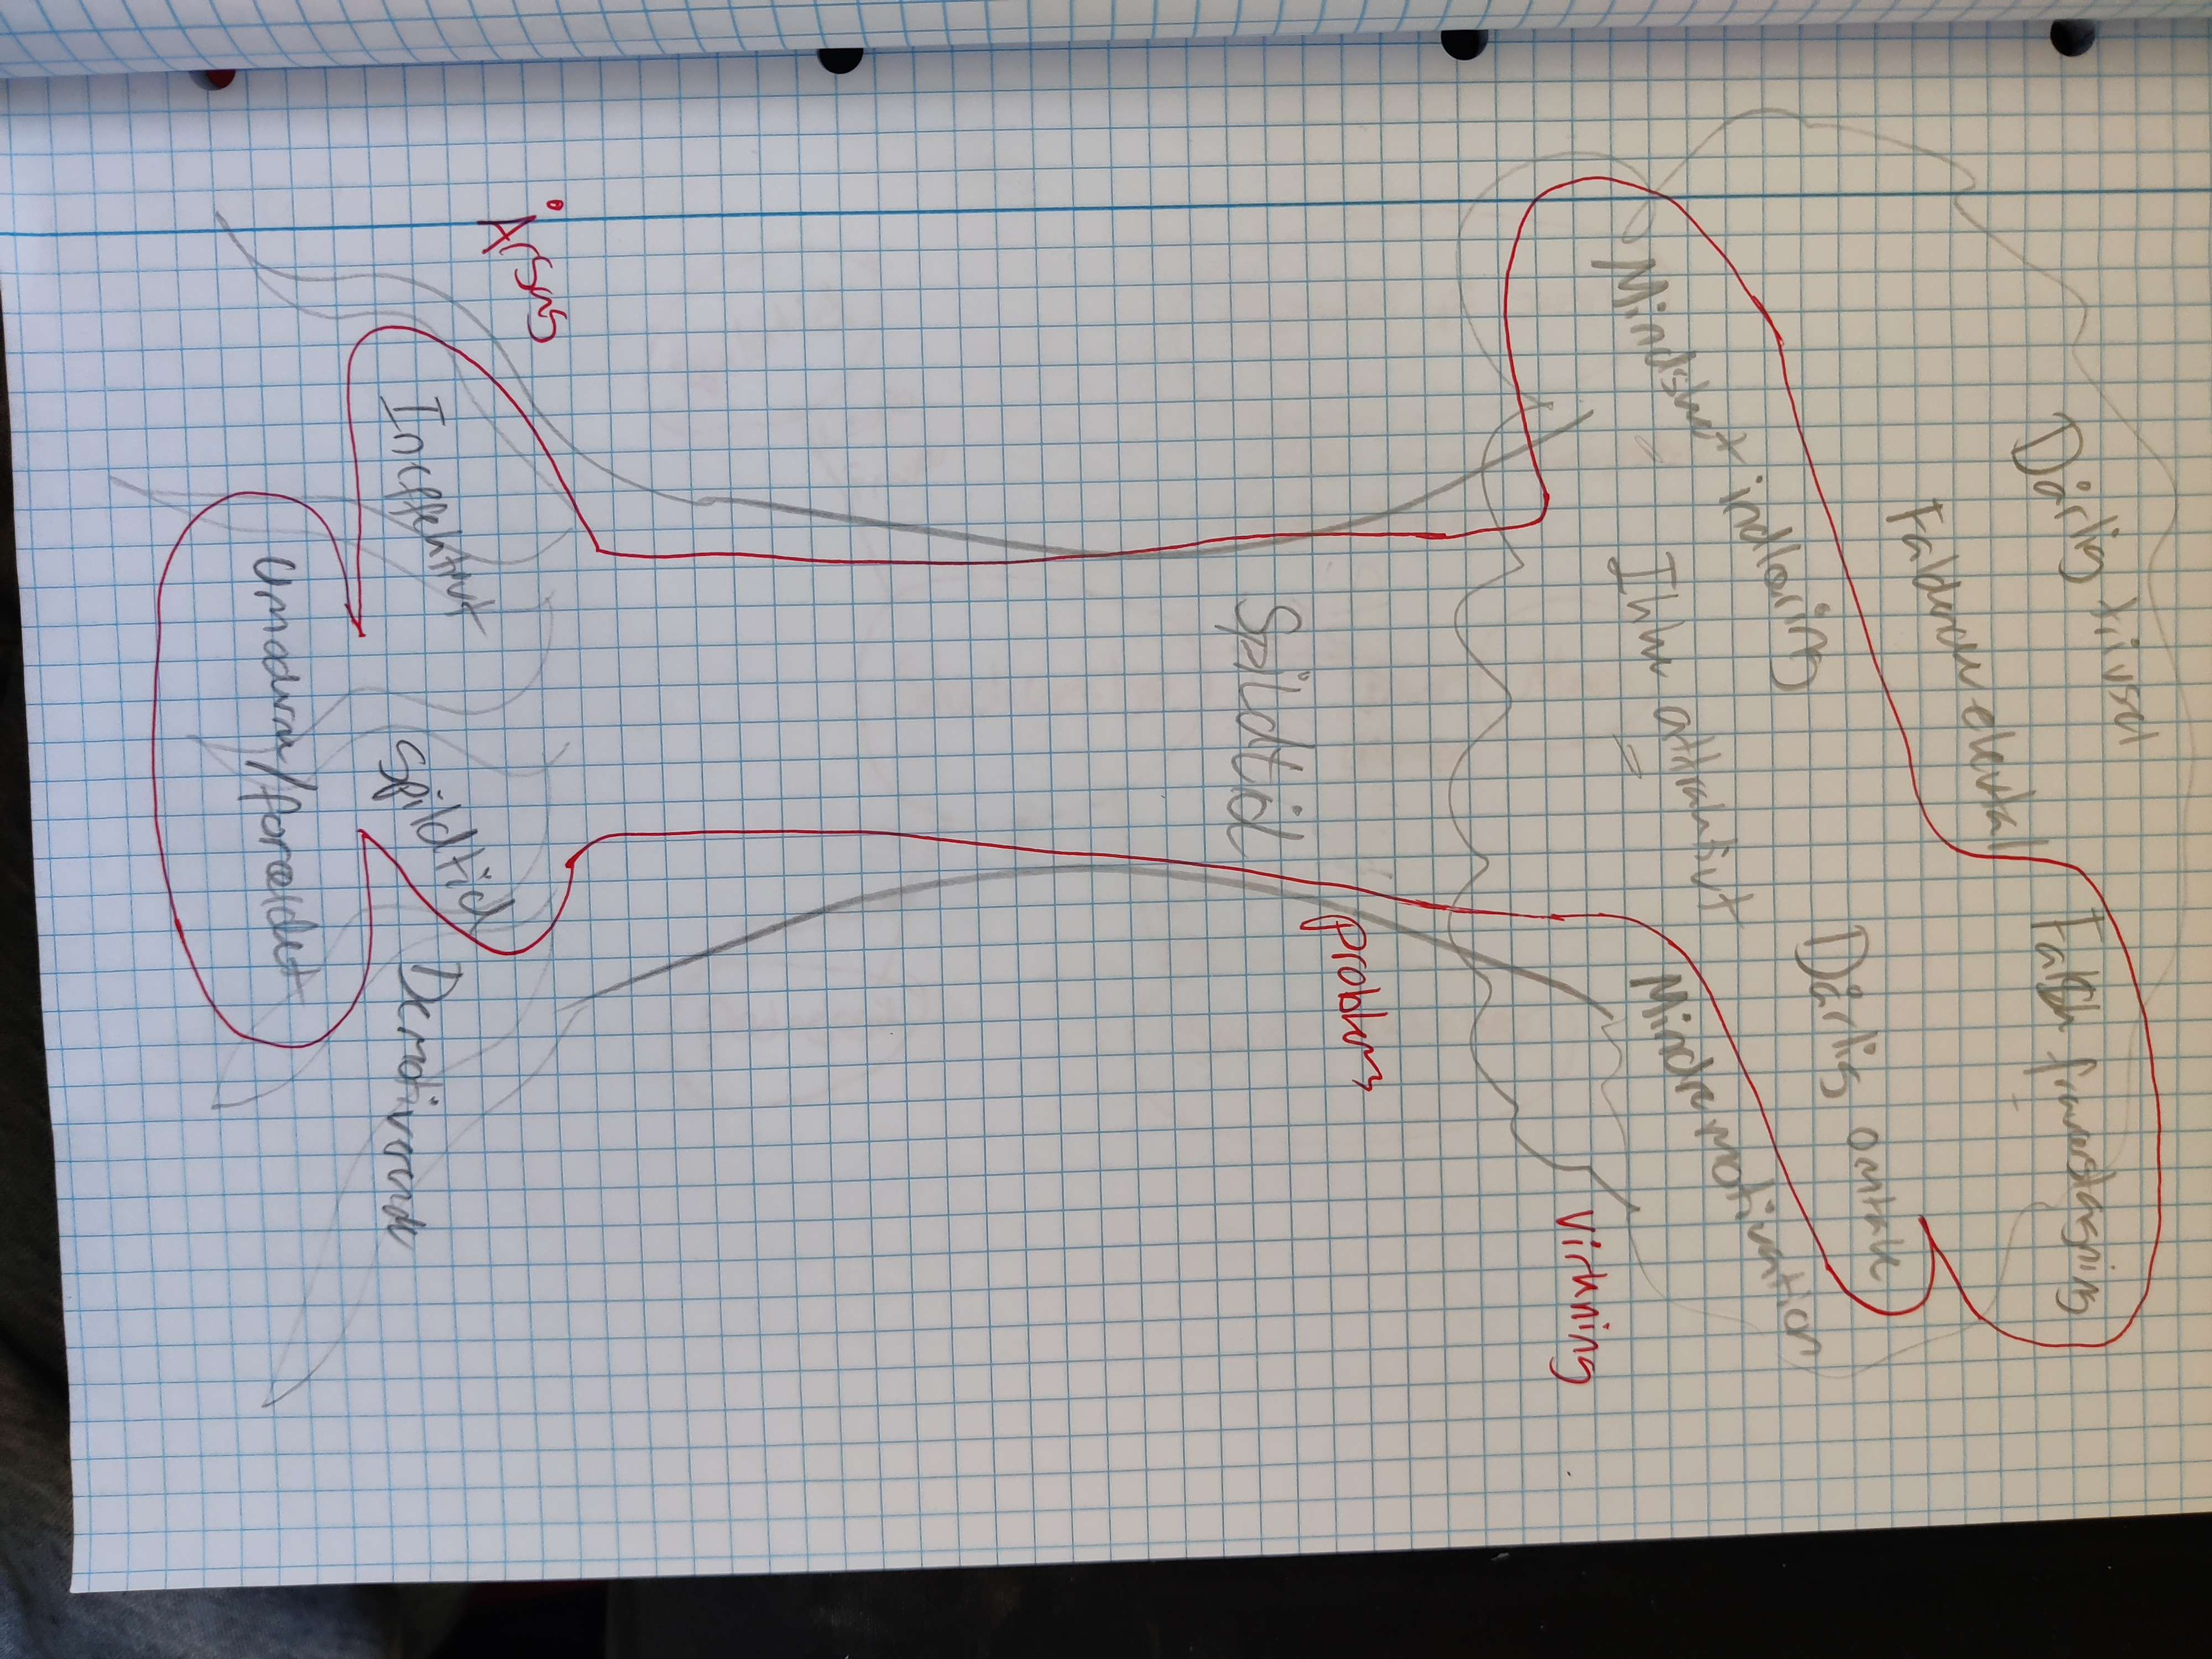
\includegraphics[angle =90]{assets/problemtrae.jpg}}
    \caption{Viser problemtræet, der blev anvendt i problemanalysen.}
\end{figure}
Et af de ineffektive systemer, vi kom i tanke om, er Lectio-applikationen, hvorefter vi har informationssøgt om emnet. Det var ikke muligt at finde nogle reele artikler om tidssplid med Lectio-applikationen, 
Da har vi forhørt os kvalitativt og snakket med flere medstuderende og flere underviserer (interessenter) som benytter sig at Lectio i deres dagligdag.
\subsection{Kvalitativ metode}
Forneden er vores overordnet indtryk af, hvordan de folk, vi har snakket med, opfatter
De har alle udtalt sig om Lectios unødvændigt komplicerede designvalg, forældede udseende og mangler. Vi snakkede bl.a. Med en underviser som udtrykte sin fustrattion over 
at det nuværende Lectio kun kan uploade et dokument ad gangen. Dette fandt vi meget mærkeligt, da vi har en udvidet viden om webudvikling, og ergo ved vi at sådan en funktion (multiupload) er utrolig nem at 
implementere og stod tilbage uforstående for, at Lectio ikke havde mulighed for så basal funktionalitet som det. Det kan også hurtigt tage fx. 10 sekunder at navigere hen til en fil og derefter uploade den, så hvis man hurtigt vil uploade fx. 10 filer, så tager dette altså 100 sekunder tilsvarende til 1 minut og 40 sekunder. 

\subsection{HV-modellen}
Herefter er HV-modellen i sammenspil med den kvalitative undersøgelse i næste kapitel, blevet anvendt til at få en ide om handlingsplanen, forbrugernes mangler og dermed potentielle produktbehov:
\paragraph{Hvad?}
    Det man skal gøre er altså at implementere basale QOL-features ved at lave et rework af Lectio. På nuværende tidspunkt er vi ikke klar over, hvem der maintainer Lectio-applikationen, ej heller hvilke tiltag de gør for at modernisere denne.
\paragraph{Hvorfor?}
    Det skal gøres, så man i fremtiden kan spare tid og tankekraft ved at gøre Lectio til en bedre IT-løsning; et system, der gør det attraktivt at anvende til at centralisere informationsdeling, således at brugere ikke søger afsides og udliciterer opgaven til 700 andre tjenester samt gør det nemtoverskueligt for brugeren at orientere sig. 
\paragraph{Hvem?}
\paragraph{Hvor?}
\paragraph{Hvornår?}
\paragraph{Hvordan?}